\chapter{Automatisch uitrollen van databases}
\section{Inleiding}
%Inleiding

\section{IMP: Framework voor installatie}
%Uitleg van IMP
\todo{Te schrijven}
%Uitleg van hoe voor elk systeem

\section{MongoDB}
In deze sectie zal 

\subsection{Werking van MongoDB}
MongoDB heeft gekozen om bij gedistribueerde database op te splitsen in 2 keuzes, een eerste is door middel van \textit{replica set}s en daarnaast door middel van \textit{shard}ing. 

\paragraph{}Bij \textit{replica set} is een master-slave configuratie van de MongoDB nodes, met de master benoemd als primary en de slaves als secondary (figuur \ref{fig:mongodb-replicaset}). De data is nog steeds beschikbaar zolang meer als de helft van de nodes beschikbaar zijn. De schrijfoperaties worden eerst naar de primary gestuurd en vervolgens door MongoDB naar de secondaries gesynchroniseerd. Ook leesoperaties worden standaard enkel naar de primary gestuurd maar dit kan aangepast worden in de configuratie. 

Met behulp van een heartbeat houden wordt de status van de verschillende nodes opgevraagd elke 10 seconden en indien de primary niet meer beschikbaar is zal een secondary gestemd worden tot primary (figuur \ref{fig:mongodb-replicaset-vote}). 

\begin{figure}[!htb]
	    \centering
    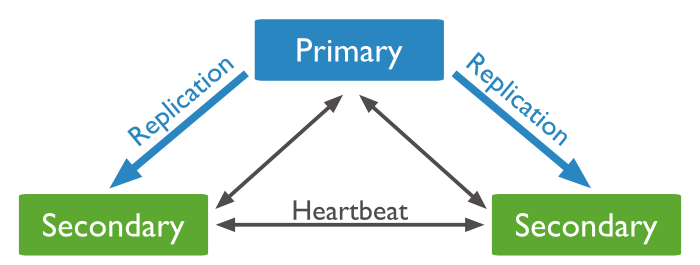
\includegraphics[width=0.7\textwidth]{img/mongodb-replica-set-primary-with-two-secondaries.png}
    \caption{MongoDB: Drie leden van een replica set met 1 master en 2 slaves. Bron: MongoDB\cite{mongodb-replicaset}}
    \label{fig:mongodb-replicaset}
\end{figure}

\begin{figure}[!htb]
	    \centering
    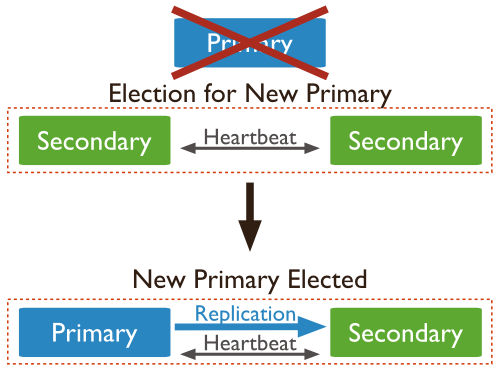
\includegraphics[width=0.7\textwidth]{img/mongodb-replica-set-trigger-election.png}
    \caption{MongoDB: Een voorbeeld van het verkiezen van een nieuwe primary bij het niet meer beschikbaar zijn van de vorige primary.  Bron: MongoDB\cite{mongodb-replicaset}}
    \label{fig:mongodb-replicaset-vote}
\end{figure}

\paragraph{} Vervolgens wordt met behulp van \textit{sharding} de data verdeeld over verschillende shards. In productie omgeving wordt aangeraden om een replica set te nemen als shard maar het is ook mogelijk om een enkele node toe te voegen. 

Voor lees- en schrijfoperaties wordt er verbinding gemaakt met mongos, dit zijn router nodes die de query naar de nodige shards stuurt. De configuratie van de shards wordt opgeslagen in 1 of 3 configuratie nodes (figuur \ref{fig:mongodb-shards}). 

\begin{figure}[!htb]
	    \centering
    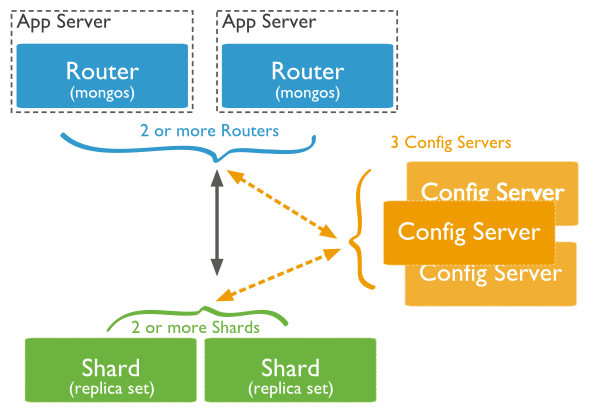
\includegraphics[width=\textwidth]{img/mongo-sharded-cluster-production-architecture.png}
    \caption{MongoDB: Een voorbeeld cluster voor productie met 2 mongos, 3 shards en 3 configuratie servers. Bron: MongoDB\cite{mongodb-shard}}
    \label{MongoDB: Een voorbeeld cluster voor productie met 2 mongos, 3 shards en 3 configuratie servers. Bron: MongoDB\cite{mongodb-shard}}
\end{figure}

De data wordt verdeeld over de verschillende shards met een door de gebruiker gedefinieerde formule, dit kan door middel van hashing of door het opsplitsen van een waarde in verschillende domeinen. 

\paragraph{} De configuratie van MongoDB is opgesplitst in 2 delen, een configuratiebestand en met behulp van de shell. Als eerste stelt men een configuratiebestand op die aan de instantie basisinformatie meegeeft zoals op welke poort, waar de database op het bestandssysteem op te slaan en welk type instantie het is (enkele node, deel van replica set, configuratie server of een mongos). 

Het opzetten van de replica sets en sharding verloopt via de shell, met behulp van een commando op een instantie die een deel is van de replica set kan de replica set opgezet worden. 
Sharding wordt opgezet door connectie te maken met een mongos en ook hier via commando shards toe te voegen, collecties aan te maken en collecties te verdelen onder shards.

Belangrijk bij sharding is dat bij het opstarten van een mongos al de verschillende configuratie servers meegegeven moeten worden, dit is de enige parameter die meegegeven moet worden in de configuratiebestanden die afhankelijk is van andere instanties. 

\subsection{Uitwerking}
Voor de uitwerking van de installatie in IMP zijn er enkele aannames genomen:
\begin{itemize}
	\item Op elke server kan hoogstens \textbf{1} MongoDB data instantie draaien, ongeachte of deze een deel is van een replica set of een alleenstaand deel is. Dit is een gegronde aanname omdat meerdere instanties betekend dat de resources gedeeld moeten worden over meerdere servers. Een nadeel hieraan is dat elke server daardoor maar lid kan zijn van 1 replica set. 
	\item Op elke server kan hoogstens \textbf{1} MongoDB config server instantie draaien. Indien er 2 configuratie instanties op de zelfde server zouden draaien, is er geen bescherming tegen het onbeschikbaar zijn van 1 server, aangezien 2 van de 3 instanties tegelijk uitvallen als deze server uitvalt. 
	\item Op elke server kan hoogstens \textbf{1} mongos instantie. Meerdere instanties bieden enkel bescherming tegen het niet meer werken van het mongos proces, maar dit kan lokaal op de computer gecontroleerd worden en indien nodig kan de service herstart worden. 
	\item Aanpassingen aan replica sets zullen afgewerkt worden met eerst het toevoegen van instanties en pas na daarna verwijderen van instantie, dit om ervoor te zorgen dat een set altijd zo veel mogelijk leden heeft. 
	\item Uitbreidingen of aanpassingen aan de verdeling van een collectie over shards is niet mogelijk maar zal geen compilatiefout geven. 
\end{itemize}

Met deze aannames is er tot het domeinmodel gekomen dat te vinden is in figuur \ref{fig:mongodb-imp-domein}. De verschillende entiteit hebben de volgende functie:
\begin{itemize}
	\item MongoDB is een server in het IMP model en is verantwoordelijk voor het installeren van de basis van MongoDB. Hierna zijn basis commando's voor connectie te maken met een MongoDB instantie beschikbaar. 
	\item MonogDBServer is een server in het IMP model en is verantwoordelijk voor het installeren van de MongoDB server. 
	\item MongoDBNode is de implementatie van een data instantie, maximaal 1 per server. Indien gelinkt met een replica set zal deze als een deel van een replica set worden geïnitialiseerd, anders als een zelfstandige instantie. 
	\item MongoDBReplicaSet is de voorstelling van een replica set, dit wordt niet aan een specifieke server toegewezen. 
	\item MongoDBReplicaSetController is verantwoordelijk om de replica set te initialiseren. Belangrijk is dat indien er een uitbreiding is van de set, de node verbonden met de controller een reeds geïnitialiseerde node is.  
	\item MongoDBConfigServer is de implementatie van een configuratie server, 1 of 3 servers zijn nodig per cluster. 
	\item MongoDBAccessServer is de implementatie van mongos, minstens 1 is nodig maar meer kunnen gebruikt worden.
	\item MongoDBShardCluster is de voorstelling van een cluster van shards, er kunnen zowel alleenstaand instanties als replica sets aan toegevoegd worden. 
	\item MongoDBShardController is verantwoordelijk om de cluster te initialiseren met de verschillende shards, databases, collecties en keys. 
	\item MongoDBDatabase is de voorstelling van een database.
	\item MongoDBCollection is de voorstelling van een collectie, indien verbonden met een cluster via een database zal deze gedeeld worden over de verschillende shards. 
	\item MongoDBKey is de wijze waarmee een collectie verdeeld wordt over de verschillende shards. 
\end{itemize}
\begin{figure}[!htb]
	    \centering
    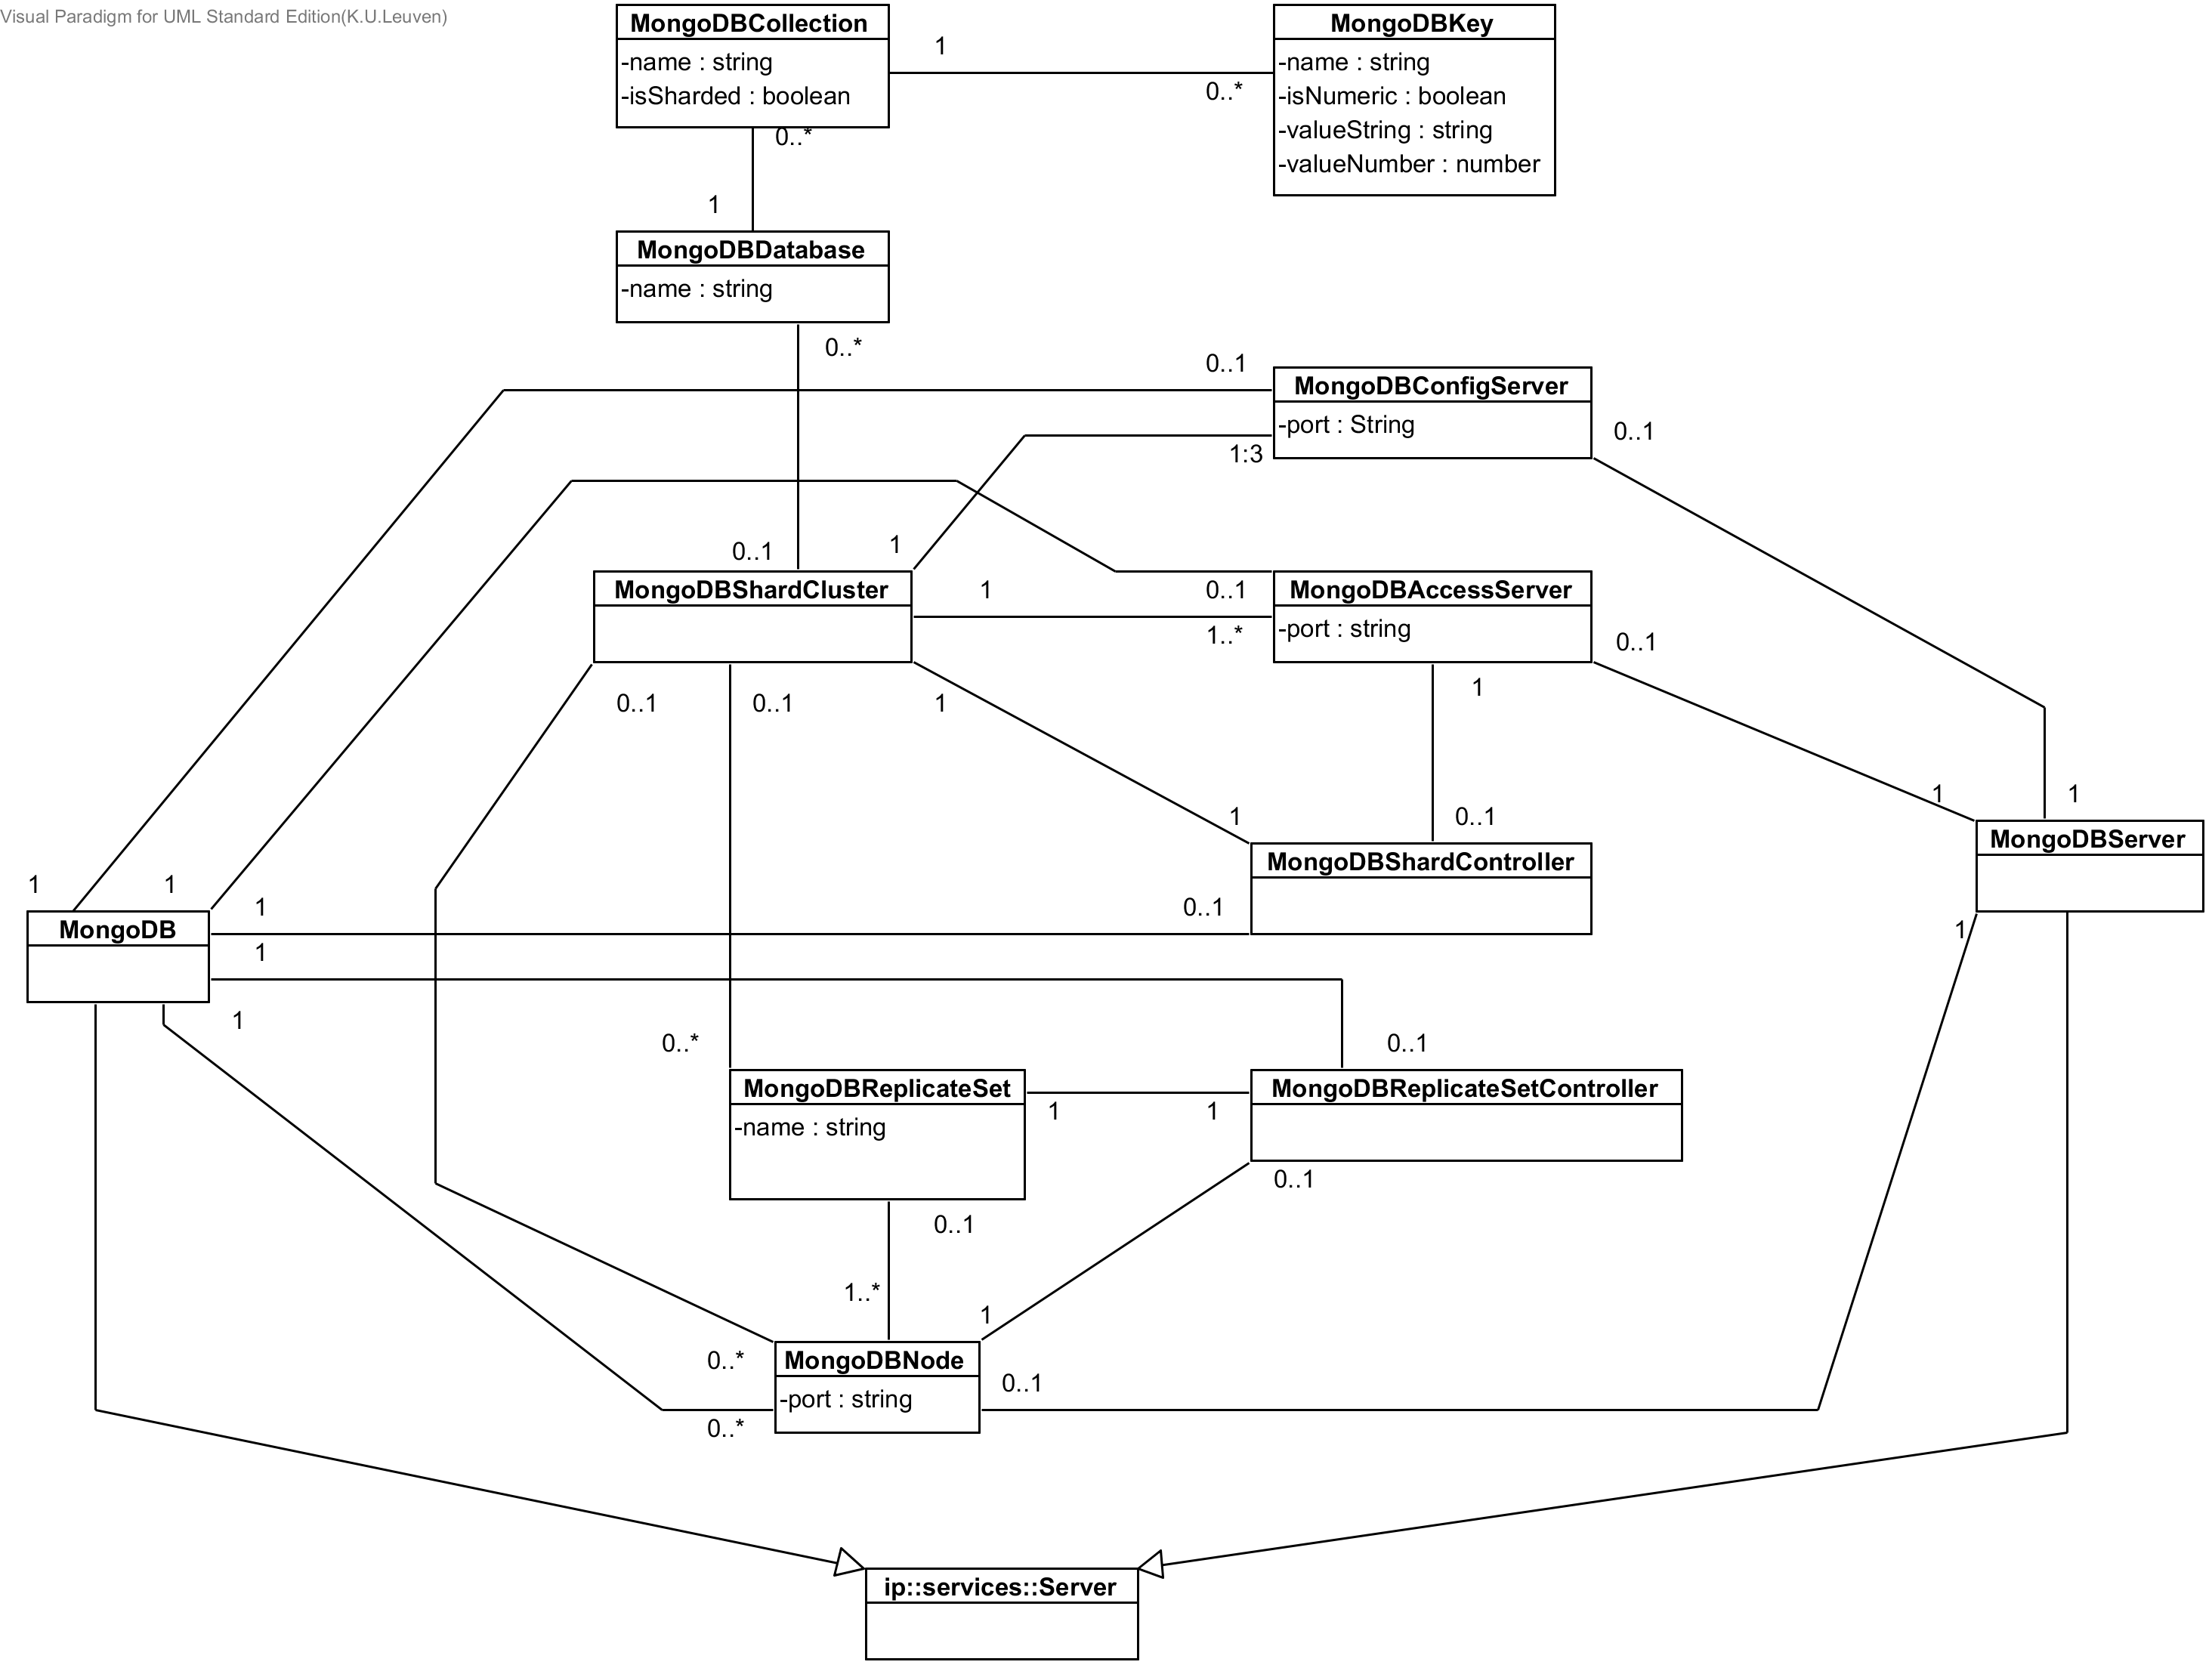
\includegraphics[width=\textwidth]{img/MongoDB-Domain.png}
    \caption{MongoDB: Het domeinmodel van de implementatie in IMP.}
    \label{fig:mongodb-imp-domein}
\end{figure}

\subsection{Resultaat}

\section{PgPool-II (PostgreSQL)}

\section{HBase}